\documentclass[border = 10pt]{standalone}
\usepackage{amsmath}
\usepackage{amssymb}
\usepackage{tikz}

\begin{document}

%% VAR
\def\rotationX{0}
\def\rotationY{-7}
\def\rotationZ{0}


\begin{tabular}{c}

\begin{minipage}{150pt}\centering
    Plano tangente ao gráfico $f:\mathbb{R}^{2}\in\mathbb{R}$ em um ponto $(x_0,y_0)$. 
\end{minipage} \vspace{2.5mm} \\

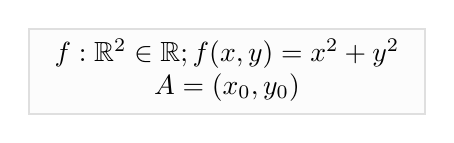
\begin{tikzpicture}
    \node [draw=gray!25,thick,fill=gray!2] {
    \begin{tabular}{c}
        $f:\mathbb{R}^{2}\in\mathbb{R};f(x,y)=x^2+y^2$ \\
        $A=(x_0,y_0)$
    \end{tabular}
    };
\end{tikzpicture} \vspace{1mm}  \\

\resizebox{400pt}{350pt}{
\begin{tikzpicture}
    [
        axis/.style={->,thick}
    ]

\begin{scope}[rotate around x=0, rotate around y=\numexpr\rotationY/2\relax,rotate around z=0]
    \coordinate (A) at (1,2,1);
    
    % (x,f(x,y),y)

    \def\verticalMax{3.5}
    \def\verticalDivisions{10}
    \def\verticalIncrement{1}

    \def\horizontalDivision{\the\numexpr360+90\relax}
    \def\horizontalIncrement{15}
    \def\horizontalInit{90}

    \foreach \i in {0, \verticalIncrement, ..., \verticalDivisions} {
        \foreach \j in {\horizontalInit, \the\numexpr\horizontalIncrement+\horizontalInit\relax, ..., \horizontalDivision} {
            \coordinate (a\i\j) at ({sqrt(\verticalMax*\i/\verticalDivisions)*sin(\j)},{\verticalMax*\i/\verticalDivisions},{sqrt(\verticalMax*\i/\verticalDivisions)*cos(\j)});
        }
    }

    \def\margim{0.5}
    %% BEGIN LEFT
    \filldraw [color=gray!25, fill=gray!2, thick] (-5,-1-\margim,3+\margim) -- (-5,4.5+\margim,3+\margim) -- (-5,4.5+\margim,-3-\margim) -- (-5,-1-\margim,-3-\margim) -- cycle;

    \draw [color=gray!25] (-5,-1,0) -- (-5,4.5,0);
    \draw [color=gray!25] (-5,0,3) -- (-5,0,-3);

    \draw [domain=-sqrt(\verticalMax):sqrt(\verticalMax), smooth, variable=\x, gray!65] plot ({-5}, {\x*\x+1}, {\x});

    \filldraw [gray] (-5,2,1) circle (1pt);
    \draw [->, gray] (-5,2,1) -- (-5,2.8944,1.4472) node[anchor=west]{$\vec v$};
    %% END LEFT

    %% BEGIN BACK
    \filldraw [color=gray!25, fill=gray!2, thick] (3+\margim,-1-\margim,-5) -- (3+\margim,4.5+\margim,-5) -- (-3-\margim,4.5+\margim,-5) -- (-3-\margim,-1-\margim,-5) -- cycle;

    \draw [color=gray!25] (0,-1,-5) -- (0,4.5,-5);
    \draw [color=gray!25] (-3,0,-5) -- (3,0,-5);

    \draw [domain=-sqrt(\verticalMax):sqrt(\verticalMax), smooth, variable=\y, gray!65] plot ({\y}, {\y*\y+1}, {-5});

    \filldraw [gray] (1,2,-5) circle (1pt);
    \draw [->, gray] (1,2,-5) -- (1.4472,2.8944,-5) node[anchor=west]{$\vec u$};
    %% END BACK

    %% BEGIN DOWN
    \filldraw [color=gray!25, fill=gray!2, thick] (-3-\margim,-2,3+\margim) -- (3+\margim,-2,3+\margim) -- (3+\margim,-2,-3-\margim) -- (-3-\margim,-2,-3-\margim) -- cycle; 

    \draw [color=gray!25] (-3,-2,0) -- (3,-2,0);
    \draw [color=gray!25] (0,-2,3) -- (0,-2,-3);

    \draw [domain=0:360, smooth, variable=\t, gray!65] plot ({sqrt(2)*sin(\t)}, {-2}, {sqrt(2)*cos(\t)});

    \filldraw [gray] (1,-2,1) circle (1pt);
    %% END DOWN

    \draw [dashed, gray!25] (1,2,1) -- (-5,2,1);
    \draw [dashed, gray!25] (1,2,1) -- (1,-2,1);
    \draw [dashed, gray!25] (1,2,1) -- (1,2,-5);

    \draw [axis] (-3,0,0) -- (3,0,0) node[anchor=west]{$x$};
    \draw [axis] (0,0,3) -- (0,0,-3) node[anchor=west]{$y$};

    \def\drawPlotWithInterval#1#2{
            \foreach \i in {0, \verticalIncrement, ..., \numexpr\verticalDivisions-\verticalIncrement\relax} {
            \foreach \j in {#1, \the\numexpr\horizontalIncrement+#1\relax, ..., #2} {
                \edef\coordsnameA{a\the\numexpr\i+\verticalIncrement\relax\j}
                \edef\coordsnameB{a\the\numexpr\i+\verticalIncrement\relax\the\numexpr\j+\horizontalIncrement\relax}
                \edef\coordsnameC{a\i\the\numexpr\j+\horizontalIncrement\relax}
                \edef\coordsnameD{a\i\j}

                \edef\colorPlot{\the\numexpr((25*\i*\j)/(\verticalDivisions*#1))+25\relax}
                \draw [fill=gray!\colorPlot] (\coordsnameA) -- (\coordsnameB) -- (\coordsnameC) -- (\coordsnameD) -- cycle;
            }
        }
    }
    
    \drawPlotWithInterval{\horizontalInit}{270}
    
    \draw [axis] (0,-1,0) -- (0,4.5,0) node[anchor=west]{$f(x,y)$};

    \drawPlotWithInterval{\the\numexpr270+\horizontalIncrement\relax}{\the\numexpr\horizontalDivision-\horizontalIncrement\relax}

    \path [fill=black!80,fill opacity=0.5] (2,0,-1) -- (-1,0,2) -- (0,4,3) -- (3,4,0) -- cycle;       
    \draw [->] (1,2,1) -- ({(2/sqrt(5))+1},{(-1/sqrt(5)+2)},{(2/sqrt(5))+1}) node[anchor=west]{$\vec n$};

    \filldraw (1,2,1) circle (1pt) node[anchor=west]{$A$};

    \draw [dashed] (1,2,1) -- (1,0,1);
    \draw [dashed] (1,0,1) -- (0,0,1);
    \draw [dashed] (1,0,1) -- (1,0,0);
    
    \filldraw (1,0,1) circle (1pt) node[anchor=west] {$a$};
\end{scope}

\end{tikzpicture}
}

\end{tabular}

\end{document}